\documentclass{pssbmac}

%%%%%%%%%%%%%%%%%%%%%%%%%%%%%%%%%%%%%%%%%%%%%%%%%%%%%%%%%%%%%%%%%%%%%%%%
%% POR FAVOR, NÃO FAÇA MUDANÇAS NESSE PADRÃO QUE ACARRETEM  EM
%% ALTERAÇÃO NA FORMATAÇÃO FINAL DO TEXTO
%%%%%%%%%%%%%%%%%%%%%%%%%%%%%%%%%%%%%%%%%%%%%%%%%%%%%%%%%%%%%%%%%%%%%%%%
\sloppy
%%%%%%%%%%%%%%%%%%%%%%%%%%%%%%%%%%%%%%%%%%%%%%%%%%%%%%%%%%%%%%%%%%%%%%%%
% POR FAVOR, ESCOLHA CONFORME O CASO
%%%%%%%%%%%%%%%%%%%%%%%%%%%%%%%%%%%%%%%%%%%%%%%%%%%%%%%%%%%%%%%%%%%%%%%%
%\usepackage[brazil]{babel} % texto em Português
\usepackage[english]{babel} % texto em Inglês

%\usepackage[latin1]{inputenc} % acentuação em Português ISO-8859-1
\usepackage[utf8]{inputenc} % acentuação em Português UTF-8
%%%%%%%%%%%%%%%%%%%%%%%%%%%%%%%%%%%%%%%%%%%%%%%%%%%%%%%%%%%%%%%%%%%%%%%%


%%%%%%%%%%%%%%%%%%%%%%%%%%%%%%%%%%%%%%%%%%%%%%%%%%%%%%%%%%%%%%%%%%%%%%%%
%% POR FAVOR, NÃO ALTERAR
%%%%%%%%%%%%%%%%%%%%%%%%%%%%%%%%%%%%%%%%%%%%%%%%%%%%%%%%%%%%%%%%%%%%%%%%
\usepackage[T1]{fontenc}
\usepackage{float}
\usepackage{graphics}
\usepackage{graphicx}
\usepackage{epsfig}
\usepackage{indentfirst}
\usepackage{amsmath, amsfonts, amssymb, amsthm, mathtools}
\usepackage{url}
\usepackage{csquotes}

\usepackage{amsmath}
\usepackage{amssymb}
% Ambientes pré-definidos
\newtheorem{theorem}{Theorem}[section]
\newtheorem{lemma}{Lemma}[section]
\newtheorem{proposition}{Proposition}[section]
\newtheorem{definition}{Definition}[section]
\newtheorem{remark}{Remark}[section]
\newtheorem{corollary}{Corollary}[section]
\newtheorem{teorema}{Teorema}[section]
\newtheorem{lema}{Lema}[section]
\newtheorem{prop}{Proposi\c{c}\~ao}[section]
\newtheorem{defi}{Defini\c{c}\~ao}[section]
\newtheorem{obs}{Observa\c{c}\~ao}[section]
\newtheorem{cor}{Corol\'ario}[section]

% ref bibliográficas
\usepackage[backend=biber,sorting=none, style=numeric-comp, maxnames=50]{biblatex}
\addbibresource{refs.bib}
\DeclareTextFontCommand{\emph}{\boldmath\bfseries}
\DefineBibliographyStrings{brazil}{phdthesis = {Tese de doutorado}}
\DefineBibliographyStrings{brazil}{mathesis = {Disserta\c{c}\~{a}o de mestrado}}
\DefineBibliographyStrings{english}{mathesis = {Master dissertation}}

%%%%%%%%%%%%%%%%%%%%%%%%%%%%%%%%%%%%%%%%%%%%%%%%%%%%%%%%%%%%%%%%%%%%%%%%


\begin{document}

%%%%%%%%%%%%%%%%%%%%%%%%%%%%%%%%%%%%%%%%%%%%%%%%%%%%%%%%%%%%%%%%%%%%%%%%
% TÍTULO E AUTORAS(ES)
%%%%%%%%%%%%%%%%%%%%%%%%%%%%%%%%%%%%%%%%%%%%%%%%%%%%%%%%%%%%%%%%%%%%%%%%
\author{Florian Echelard}
\title{Pocket Lipid Interaction}

\criartitulo
%%%%%%%%%%%%%%%%%%%%%%%%%%%%%%%%%%%%%%%%%%%%%%%%%%%%%%%%%%%%%%%%%%%%%%%%


%%%%%%%%%%%%%%%%%%%%%%%%%%%%%%%%%%%%%%%%%%%%%%%%%%%%%%%%%%%%%%%%%%%%%%%%
% TEXTO
%%%%%%%%%%%%%%%%%%%%%%%%%%%%%%%%%%%%%%%%%%%%%%%%%%%%%%%%%%%%%%%%%%%%%%%%

\begin{abstract}
{\bf Summary}. \\
Using Voronota and Pytorch to investigate interactions
\end{abstract}

\section{Introduction}

Lipid transfer proteins (LTPs) are Peripheral Membrane Proteins that transfer a lipid from a donor membrane to an
acceptor membrane with specificity for each membrane, and for the lipid. Their structure involves an hydrophobic cavity that covers the entire lipid.
Lipidomics experiments yielded novel results of LTPs binding to liposomes. Using interaction data detailing the lipid composition of the membrane bound by proteins of this family, we will analyze in detail the properties and mechanisms we can outline from these experiments. 
As the experiment lay out genes for proteins and profiles for lipid, some preprocessing for selecting the data is necessary. The approach we took is structural for the protein, using Graph Neural Network to interpret features, using a pytorch library that focuses on this \cite{pytorch} \cite{pytorchgeo}. For the lipid we do not have the complex (meaning the protein and lipid bound in one structure), so we use the SMILES 1D encoding as the lipid structure, with a Chemical Language Model specifically trained on small molecules \cite{molformer}.
\begin{figure}[H]
    \centering
    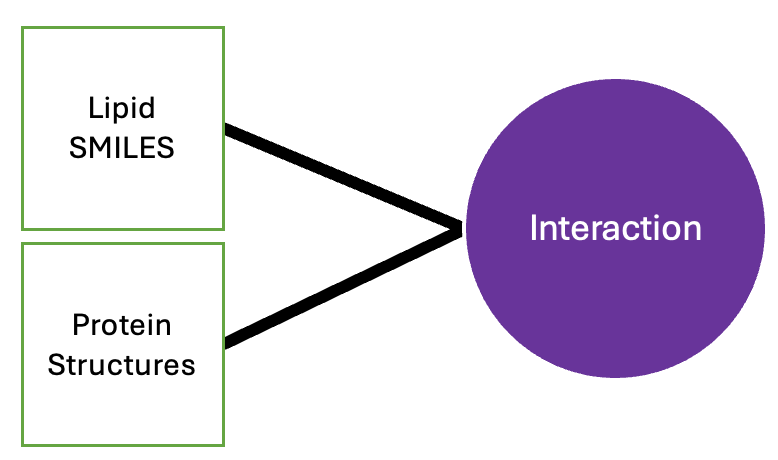
\includegraphics[width=0.35\linewidth]{figures/Screenshot 2025-06-18 at 11.09.04.png}
    \caption{Goal of the study, predict the interaction (yes/no) using two different representations and multimodal learning}
    \label{fig:schema}
\end{figure}
\section{Data}

\subsection{Protein Structures}
Selected structures without mutations (\textbf{data/structures/possible\_pdbs.numbers}) from the PDB, AFDB if not available. Based on Uniprot Family and Domain annotation (mostly from PROSITE) (\textbf{data/structures/raw})

\subsection{Lipid SMILES}
Using the description of the lipid head group and chain (\textbf{data/LTP-lipid\_interaction.csv}) from Mass Spectrometry data. We then submit REST API requests to LipidMaps (\textbf{data/lipid\_maps\_fetch.py})  We get SMILES format back for the molecules, which are one of the ways to annotate 2D graphs in one dimension. \cite{lipidmaps}

\subsection{Interactions}
All positive interactions are present in (\textbf{data/LTP-lipid\_interaction.csv}), each line is a recorded lipid inside of a LTP \cite{acg}.

\section{Preprocessing}

Additional information must be generated to identify the pocket and its properties.

\subsection{Duplicates}

In the original dataset, several lines pertains to the same interaction, but from different experiments. A choice was made to combine profiles with no sidechain description with profiles that do have these details. (\textbf{data/Processed\_dataset.csv})

\subsection{Negative Interactions}
The previous iteration of the training used every LTP-lipid pair possible that is not in the original dataset as a negative interaction. This approach may not be best, especially now considering that we went from 1137 positive and 14000 negative interaction to 751 positive interactions.

\subsection{Voronota}

Using the Voronota software's \cite{voronota} voronota-pocket to annotate pockets in the .pdb's b-factor column(\textbf{preprocessing/voronota\_parameter\_per\_ltp.xlsx}) instead of the whole annotated structures (\textbf{data/structures/voronota}). This is to verify the annotation. \\
 Parameters can be changed depending on the type of pocket to consider. LTPs are known to possess large hydrophobic pockets, which is why it is important to test different sets of parameters that show a good cutoff between the hydrophobic pocket and the grooves around the surface. To select a set of parameter that accomodates this criteria, we use visual inspection on the annotated structures with pymol, to verify that this set is satisfactory for all proteins in our dataset.
To generate the graphs used in the training, we use a script from voronota-js (\textbf{preprocessing/voronota-js-receptor-data-graph})  \\

These graphs (\textbf{data/graphs}) are separated into nodes and edges files, for atom without prefix, and for amino acids with the "coarse" prefix. There are features relevant to the atom and amino acid chemistry, as well as descriptors computed based on the geometry of the protein (see details on : \textit{https://github.com/kliment-olechnovic/generating-graphs-of-protein-receptors}). \\

There were discussions as to which level of detail is better to train the model. as our current dataset is only composed of 35 protein structures, the atomic level description might be too noisy to construct a good representation. Combining the geometric description of coarse-grained atoms into amino acids is a promising avenue, and this level of definition is important as it is the same dimension for ESM3/PLMs tokens.


\subsection{Lipid Embedding}

To use the lipid as input, we first need to encode its SMILES into tokens from a pretrained network \cite{molformer}. We make a list of our SMILES (\textbf{embed\_smiles.py}). Here we use Molformer, and use a modified script to encode our data (\textbf{preprocessing/frozen\_embedding.py}) inside of the git directory (https://github.com/IBM/molformer/tree/main/notebooks/pretrained\_molformer). The dimension of a SMILES embedded sequence is $[N,768]$. An additional token is added at the beginning of the sequence, the  $<CLS>$ token, that can be used instead of pooling on the whole sequence, as it was used in training to represent the whole sequence with attention. 

\subsection{Protein Embedding}

The voronota graph script featurises a lot of aspects of the structure, but during tests, we weren't able to learn any task by only using geometric and chemical descriptors. So by coarsegraining on amino acids and using Protein Language Model embeddings of the sequence and projecting it on the structure, results were a bit better. So we use ESM3 \cite{esm3} to embed these sequences (\textbf{preprocessing/EmbedProtein.py}). The current available model for generating embeddings based on the sequence is "esm3-sm-open-v1" (https://huggingface.co/EvolutionaryScale/esm3-sm-open-v1).  \\

The embeddings are accessible in the (\textbf{data/embedding\_ESM3}) directory, compared to the coarse-grained residue nodes of the graph, the model adds two token, a $<BOS>$ at the beginning and $<EOS>$ at the end. To make sure the token dimensions matches with the coarse grained graph nodes, it is better to remove the before concatenating them with Voronota descriptors. The dimension of a sequence is $[N,1536]$ so to keep the relative importance of other features the latent dimension should be projected by a linear layer before concatenation with other features.

\section{Achitecture}

\subsection{Lipid}

As we are using a pre-trained network embedding as our input, we can use feed forward or self-attention layers to train our representation. We consider the lipid as tokens within a graph in our approach, but we do not have specific edges, so it is initially considered fully connected. To test this part of the architecture, we have a task to predict a head group from the embedding. \textbf{(architecture/toy\_task/LipPred.py)}

\subsection{Protein}

The protein graph is sparse, and we have geometric and chemical features for every atom, which can be coarse grained into amino acids. We can then combine embeddings from PLMs. To create a representation for the protein, we can use a combination of Graph Convolutional Networks and Graph Attention Network. To test this part of the architecture, we can predict the domain type the structure is part of. \textbf{(architecture/toy\_task/ProtPred.py)}

\subsection{Cross Attention}

To have the two representations communicate and predict a property, we use Cross Attention. As multimodal networks implementation depends on the data used, several approaches and combination of data have to be tested.

The original design of the cross attention relied on an antibody interaction deep learning model, that uses multimodal input and a combination of cross and self attention to create a representation to update the relative position of the complex (\tiny\textit{https://www.mlsb.io/papers\_2022/End\_to\_end\_accurate\_and\_high\_throughput\_modeling\_of\_antibody\_antigen\_complexes.pdf}).
\normalsize

\section{Training}

\subsection{Loss}

As the prediction for the interaction is binary, Binary Cross Entropy Loss seems the most appropriate. 

\subsection{Data Split}

Several approaches are possible for data splitting. The domain types are unevenly distributed, there is less protein diversity than lipids. So we can approach splitting the train, validation, and test by looking at the domain family of the protein, or the head group of the lipid. If we want to test for generalization, we can leave out a whole class of proteins or lipid, as their representation alone should allow to extrapolate on new data. An approach of randomised sampling will very probably encompass all the proteins, but can sideline some lipids. This can be interesting for early tests.

Keep in mind that the dataset reveals only positive interactions. The negative interactions are generated based on the rule that if a lipid was not seen as transported by a certain protein in the experiments, it's that it doesn't. This assomption brings about a huge bias, considering that you may want to restrict negative interactions to a comparative number to the positive one during training. It means that based on your sampling of "negative" interactions, the model will yield different results.

Another bias of unknown impact is the fact that the original dataset does not include detailed structure for the lipid, meaning that most of the time the structure of the chains is uncertain, both their carbon length, and the localisation of the unsaturation. It means that the SMILES used are similar at best to the actual molecule seen during mass spectrometry experiments, but every data point probably has slight difference from the ground truth in some of the aspects described here. Which cannot be adressed unless additional experiments are made for all the systems and interactions.

The batch object comes from torch\_geometric.data.Data(), both for the protein graph and the lipid. This allows to batch several graphs together by using an adjacency matrix.
%%%%%%%%%%%%%%%%%%%%%%%%%%%%%%%%%%%%%%%%%%%%%%%%%%%%%%%%%%%%%%%%%%%%%%%%
% REFS BIBLIOGRÁFICAS
% POR FAVOR, NÃO ALTERAR
%%%%%%%%%%%%%%%%%%%%%%%%%%%%%%%%%%%%%%%%%%%%%%%%%%%%%%%%%%%%%%%%%%%%%%%%
\printbibliography
%%%%%%%%%%%%%%%%%%%%%%%%%%%%%%%%%%%%%%%%%%%%%%%%%%%%%%%%%%%%%%%%%%%%%%%%

\end{document}




